% Download from : https://www.acm.org/publications/proceedings-template
% old template https://www.acm.org/publications/proceedings-template-16dec2016

\documentclass[sigconf]{acmart}
%\documentclass[10pt,sigconf]{acmart}

\usepackage{booktabs} % For formal tables


%\usepackage{times}
%
%\usepackage{shadow}
%\usepackage{hhline}
%\usepackage{latexsym}
%\usepackage[T1]{fontenc}
%\usepackage{xspace}
%\usepackage{soul}
%\usepackage[dvipsnames]{xcolor}
%\usepackage{booktabs}
%\usepackage{graphicx}
%\usepackage[protrusion=true,expansion=true]{microtype}
%\usepackage{fancyhdr}
%\usepackage{tabularx}
%\usepackage{comment}
%\usepackage{cite}
%\usepackage{enumitem}
%% \usepackage{flexisym} % DH: for \textprime
%\usepackage{placeins}  % DH: for  \FloatBarrier

\newcommand{\tl}{TensorLayer }
\hyphenation{TensorLayer}

% Copyright
%\setcopyright{none}
%\setcopyright{acmcopyright}
%\setcopyright{acmlicensed}
\setcopyright{rightsretained}
%\setcopyright{usgov}
%\setcopyright{usgovmixed}
%\setcopyright{cagov}
%\setcopyright{cagovmixed}


%% DOI
%\acmDOI{10.475/123_4}
%
%% ISBN
%\acmISBN{123-4567-24-567/08/06}

%Conference
%\acmConference[ACMMM]{ACM Multimedia}{Oct 2017}{Mountain View, CA USA} 
%\acmYear{2017}
%\copyrightyear{2017}




%\acmPrice{15.00}



\begin{document}
	

\title{TensorLayer: A Versatile Library for Efficient Deep Learning Development}
%\titlenote{Produces the permission block, and
%  copyright information}
%\subtitle{Extended Abstract}
%\subtitlenote{The full version of the author's guide is available as
%  \texttt{acmart.pdf} document}


%\author{Ben Trovato}
%\authornote{Dr.~Trovato insisted his name be first.}
%\orcid{1234-5678-9012}
%\affiliation{%
%  \institution{Institute for Clarity in Documentation}
%  \streetaddress{P.O. Box 1212}
%  \city{Dublin} 
%  \state{Ohio} 
%  \postcode{43017-6221}
%}
%\email{trovato@corporation.com}
%
%\author{G.K.M. Tobin}
%\authornote{The secretary disavows any knowledge of this author's actions.}
%\affiliation{%
%  \institution{Institute for Clarity in Documentation}
%  \streetaddress{P.O. Box 1212}
%  \city{Dublin} 
%  \state{Ohio} 
%  \postcode{43017-6221}
%}
%\email{webmaster@marysville-ohio.com}
%
%\author{Lars Th{\o}rv{\"a}ld}
%\authornote{This author is the
%  one who did all the really hard work.}
%\affiliation{%
%  \institution{The Th{\o}rv{\"a}ld Group}
%  \streetaddress{1 Th{\o}rv{\"a}ld Circle}
%  \city{Hekla} 
%  \country{Iceland}}
%\email{larst@affiliation.org}
%
%\author{Valerie B\'eranger}
%\affiliation{%
%  \institution{Inria Paris-Rocquencourt}
%  \city{Rocquencourt}
%  \country{France}
%}
%\author{Aparna Patel} 
%\affiliation{%
% \institution{Rajiv Gandhi University}
% \streetaddress{Rono-Hills}
% \city{Doimukh} 
% \state{Arunachal Pradesh}
% \country{India}}
%\author{Huifen Chan}
%\affiliation{%
%  \institution{Tsinghua University}
%  \streetaddress{30 Shuangqing Rd}
%  \city{Haidian Qu} 
%  \state{Beijing Shi}
%  \country{China}
%}
%
%\author{Charles Palmer}
%\affiliation{%
%  \institution{Palmer Research Laboratories}
%  \streetaddress{8600 Datapoint Drive}
%  \city{San Antonio}
%  \state{Texas} 
%  \postcode{78229}}
%\email{cpalmer@prl.com}
%
%\author{John Smith}
%\affiliation{\institution{The Th{\o}rv{\"a}ld Group}}
%\email{jsmith@affiliation.org}
%
%\author{Julius P.~Kumquat}
%\affiliation{\institution{The Kumquat Consortium}}
%\email{jpkumquat@consortium.net}

% The default list of authors is too long for headers}
%\renewcommand{\shortauthors}{B. Trovato et al.}

\author{Hao Dong, Akara Supratak, Luo Mai, Fangde Liu, Axel Oehmichen, Simiao Yu, Yike Guo }%
\renewcommand{\shortauthors}{H. Dong et al.}

%\\ %SUBMITTED to ACM MULTIMEDIA 2017 OPEN SOURCE SOFTWARE COMPETITION}
\affiliation{\institution{Imperial College London}}
\email{{hao.dong11, akara.supratak12, luo.mai11, fangde.liu, axelfrancois.oehmichen11, simiao.yu13, y.guo}@ic.ac.uk}

\begin{abstract}
Recently we have observed emerging uses of deep learning techniques
in multimedia systems.
Developing a practical deep learning system is arduous and complex.
It involves labor-intensive tasks for constructing sophisticated neural networks, 
coordinating multiple network models, and managing a large amount of training-related data. 
%The development efficiency is determined not only by the performance of training engines, but also by the richness of abstracted functions for managing neural networks, training data and parallel computation. 
To facilitate such a development process, we propose
\tl which is a Python-based versatile deep learning library.
\tl provides high-level modules that abstract sophisticated operations towards 
neuron layers, network models, 
training data and dependent training jobs. In spite of offering simplicity, 
it has transparent module interfaces that allows 
developers to flexibly embed low-level controls within a backend engine,
with the aim of supporting fine-grain tuning towards training.
Real-world cluster experiment results show that \tl is able to achieve competitive performance and scalability
in critical deep learning tasks.
%Specifically, it contains (1) a layer module
%that provides numerous reference neuron layers for building deep learning models,
%(2) a neural network module that achieves fine-grain control of network life-cycle,
%(3) a dataset module that helps developers create
%training datasets (offline or online) in a flexible fashion,
%and (4) a workflow module
%that supports transparent scaling-out computations for complex training requests. 
\tl was released in September 2016 on GitHub. Since after, it soon become one of the most popular
open-sourced deep learning library used by researchers and practitioners. 


%\begin{keywords}
%	One, two, three, four, five
%\end{keywords}
\end{abstract}

\pagestyle{empty} % Hao remove header

%%
%% The code below should be generated by the tool at
%% http://dl.acm.org/ccs.cfm
%% Please copy and paste the code instead of the example below. 
%%
%\begin{CCSXML}
%<ccs2012>
% <concept>
%  <concept_id>10010520.10010553.10010562</concept_id>
%  <concept_desc>Computer systems organization~Embedded systems</concept_desc>
%  <concept_significance>500</concept_significance>
% </concept>
% <concept>
%  <concept_id>10010520.10010575.10010755</concept_id>
%  <concept_desc>Computer systems organization~Redundancy</concept_desc>
%  <concept_significance>300</concept_significance>
% </concept>
% <concept>
%  <concept_id>10010520.10010553.10010554</concept_id>
%  <concept_desc>Computer systems organization~Robotics</concept_desc>
%  <concept_significance>100</concept_significance>
% </concept>
% <concept>
%  <concept_id>10003033.10003083.10003095</concept_id>
%  <concept_desc>Networks~Network reliability</concept_desc>
%  <concept_significance>100</concept_significance>
% </concept>
%</ccs2012>  \textsl{}
%\end{CCSXML} 
%
%\ccsdesc[500]{Computer systems organization~Embedded systems}
%\ccsdesc[300]{Computer systems organization~Redundancy}
%\ccsdesc{Computer systems organization~Robotics}
%\ccsdesc[100]{Networks~Network reliability}

\keywords{Deep Learning, Reinforcement Learning, Parallel Computation, Computer Vision, Natural Language Processing, Data Management}


\copyrightyear{2017} 
\acmYear{2017}
\setcopyright{acmlicensed}
\acmConference{MM '17}{October 23--27, 2017}{Mountain View, CA, USA}\acmPrice{15.00}\acmDOI{10.1145/3123266.3129391}
\acmISBN{978-1-4503-4906-2/17/10}

\maketitle

\section{Introduction}

% {\color{blue}
% \textbf{Words and Problem Definition}\\
% 1. Learning system > Network (include model architecture and parameters) > Layer \\
% 2. Some layers have parameters (fully-connected layer, convolutional layer etc), some layers do not have parameters (pooling layer, dropout), but have other behaviour.\\
% 3. Why parameter sharing is important?\\ 
% - In complex deep learning applications, different networks or layers may have different behaviour in different time, 
% or some layers have to be reused, like siamese network~\cite{} which the same CNN network will be used to encode two images.
% %Another example is generative neural network (GAN)~\cite{}, the input of discriminator 
% \\
% 4. Concept of TL layer.\\
% - All layers have 4 properties in common: %$http://tensorlayer.readthedocs.io/en/latest/modules/layers.html#understand-basic-layer$
% \\
% - Simple example: %$http://tensorlayer.readthedocs.io/en/latest/modules/layers.html#a-simple-layer$
% \\
% - This layer design make sure all layer have all parameters, dropout probabilities and layers' outputs of its previous layers, e.g. the latest layer is the whole network. This design helps to build complex learning system.
% \\
% - More details about concept of TL layer please check my $"\_previous\_draft.pdf"$.\\
% 6. Concept of TensorDB\\
% - Everything (including job, network model and its parameters) are data.\\
% - More details about concept of TensorDB please check $\_tensordb\_paper.pdf$.
% }

%Deep learning has been widely used in today's multimedia systems.
Recently we have observed the prosperity of applying deep learning into multimedia systems.
Important applications include achieving visual recognition using convolution neural networks (CNN) (e.g., object recognition \cite{krizhevsky2012imagenet} and image generation \cite{radford2015dcgan}), natural language understanding using recurrent neural networks (RNN) \cite{mikolov2010recurrent}
and machine strategic thinking using deep reinforcement learning (DRL) \cite{mnih2015human}.
Such a prosperity has led to a booming of deep learning 
frameworks including TensorFlow \cite{abadi2016tensorflow}, MXNet \cite{chen2015mxnet}, Torch \cite{collobert2002torch} and CNTK \cite{seide2016cntk}.
Developing a deep learning system typically starts with a rigorous search for an optimal neural network. 
A typical neural network consists of stacked neuron layers such as dropout \cite{srivastava2014dropout}, batch normalization \cite{ioffe2015batch}, CNN and RNN. Developers rapidly evaluate varied networks 
by utilizing rich reference layer implementations imported from open source libraries including
Caffe \cite{jia2014caffe}, Keras \cite{chollet2015}, Theano \cite{bergstra2010theano}, Sonnet \cite{sonnet} and TFLearn \cite{tflearn2016}.

Deep learning systems are increasingly interactive~\cite{amershi2014power}. 
This has led to three transitions in their development landscape.
Firstly, datasets are becoming dynamic. The emergence of 
learning systems that involve feedback loops, e.g., DRL and active learning \cite{gal2017deep},
has spawn numerous requests for manipulating, consolidating and querying datasets.
Secondly, models are becoming composite. To achieve precise recognition, a deep neural network, e.g., dynamic neural networks \cite{andreas2016learning} and generative adversarial networks (GANs)~\cite{radford2015dcgan},
can need to activate varied neuron layers according to input features.
Thirdly, training is becoming continuous. Samples, features, 
human insights, and operation experiences 
can be produced even after deployment. 
It thus becomes necessary to constantly optimize the hyper-parameters
of a neural network by supporting human-in-the-loop.

% I am not understanding that phrase:
The growing interactivity complicates deep learning development.  
Developers have to spend many 
cycles on integrating components for experimenting neural networks, managing intermediate training states, 
organizing training-related data, and enabling hyper-parameter tuning in responses to varied events. 
To reduce required cycles, we argue for an integrative development approach where 
the complex operations towards neural networks, states, data, and hyper-parameters are abstracted
and provided within complementary modules. 
This spawns an unified environment where developers are able to efficiently explore
ideas through high-level module operations, and apply customizations to modules
only if necessary. This approach does not intend to create module lock-in. Instead,
modules are modelled minimal single-function blocks that share an interaction interface, which
allows easy plug-ins of user-defined modules.

\tl is a community effort to achieve this vision. It is a modular
Python library that provides easy-to-use modules to facilitate researchers
and engineers in developing complex deep learning systems. Currently, it has 
(1) a \emph{layer} module that provides reference implementation of neuron layers 
which can be flexibly interconnected to architect neural networks,
(2) a \emph{model} module that can help manage the intermediate states incurred throughout a model life-cycle,
(3) a \emph{dataset} module that manages training data which can be used by both offline and online learning systems, 
and (4) a \emph{workflow} module that supports asynchronous scheduling and failure recovery for concurrent training jobs.
In addition to using high-level module APIs, \tl users are allowed to offload low-level functions
into execution backends to achieve fine-grain controls towards a training process. This transparent interface design is 
particular useful when addressing domain-specific problems. 

\tl implementation is optimized for performance and scalability. It adopts TensorFlow as the distributed training and inference engine. 
Delegation into TensorFlow exhibits negligible overhead. In addition, \tl uses MongoDB as the storage backend.
This backend is augmented with an efficient stream controller
for managing unbounded training data.  
To enable automation, this controller is able to 
batch results from a dataset query 
and spawns batch training tasks accordingly. 
For efficiently handling large data objects like videos, \tl uses GridFS as a blob backend, and makes
MongoDB act as an sample indexer. Finally, \tl implements
an agent pub-sub system to achieve asynchronous training workflow. Agents
can be placed onto various kinds of machines and
subscribe to independent tasks queues.
These queues are managed by in reliable storages so that failed tasks can be replayed automatically.

In contrast to other TensorFlow-based libraries such as Keras and TFLearn, 
TensorLayer permits straightforward low-level controls within the execution of layers and neural networks. 
In addition, it provides extra dataset and workflow modules to free users from labor-intensive 
data pre-processing, post-processing, module serving and data management tasks. Last but not least,
\tl does not create library lock-in. Its unified module interaction interface can accept
layers and networks imported from Keras and TFLearn in a non-invasive manner.

\tl was released on Github~\footnote{\url{https://github.com/zsdonghao/tensorlayer}} in September 2016, and soon become one of the most popular 
open-sourced deep learning libraries \cite{dlranking2017}. By July 2017, it has received more than 1900 stars and has formed an 
active development community. We demonstrate its 
effectiveness through real-world applications, where \tl are used to implement
DRL, GANs, model cross-validation and hyper parameter optimization~\cite{bergstra2012random}. These applications were previously challenging 
to develop and requires expensive development effort for integrating storage, fault-tolerance,
computations and cluster management components. The use of \tl significantly accelerates such a process. 

%As using layer in layer out design, all other TensorFlow wrappers and ops can be merged into TensorLayer by using LambdaLayer.

\section{Architecture}

We describe the architecture of \tl in Figure~\ref{fig:architecture}.
A deep learning developer 
writes a multimedia system using helper functions from \tl.
These functions range from providing and importing layer implementations,
to building neural networks, to managing states involved throughout model life-cycles, 
to creating online or offline datasets, and to writing a parallel training plan.  
These functions are grouped into four modules: layer, network, dataset, and workflow. 
In the following, we describe these modules, respectively.

\begin{figure}
	\centering % trim={<left> <lower> <right> <upper>}
%	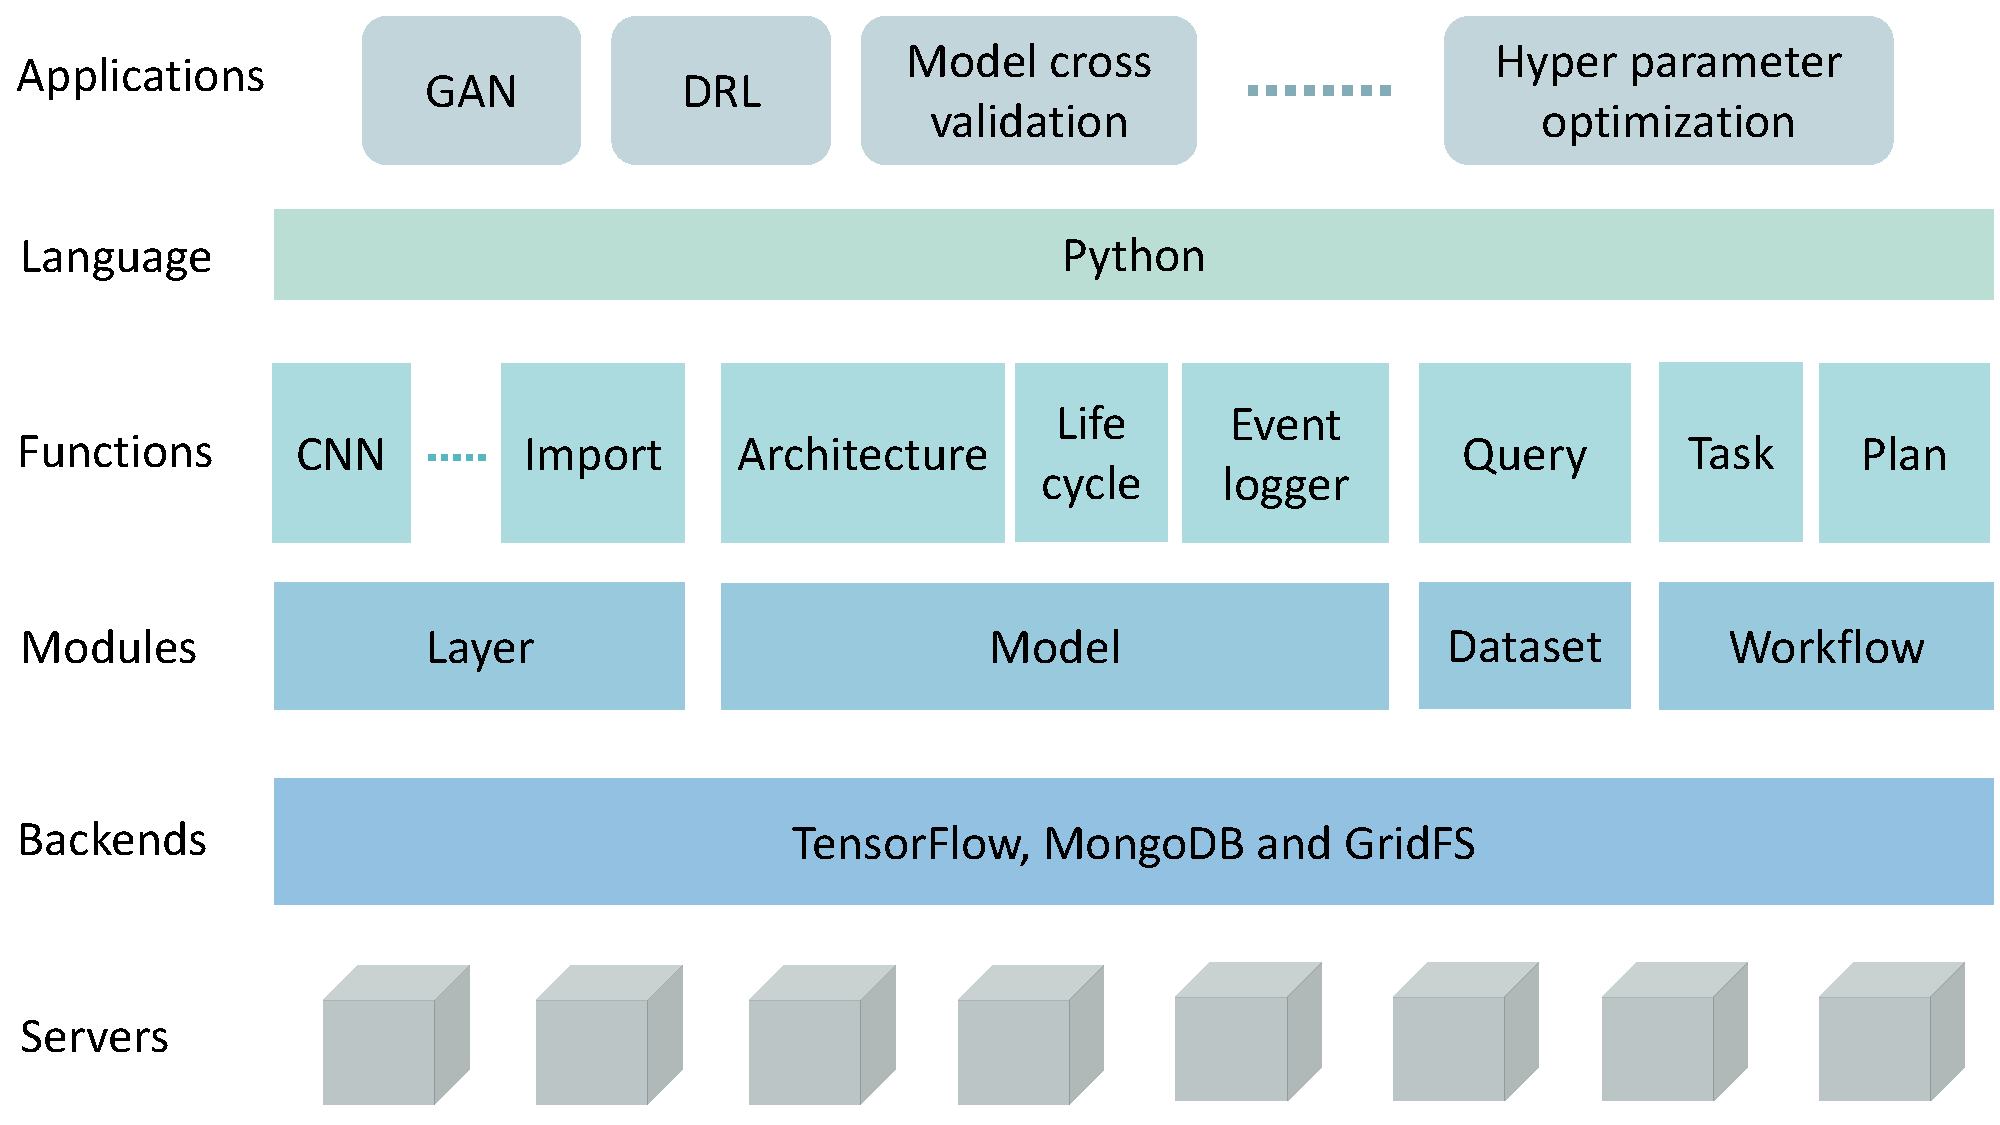
\includegraphics[width=0.46\textwidth]{figures/architecture.pdf}
%	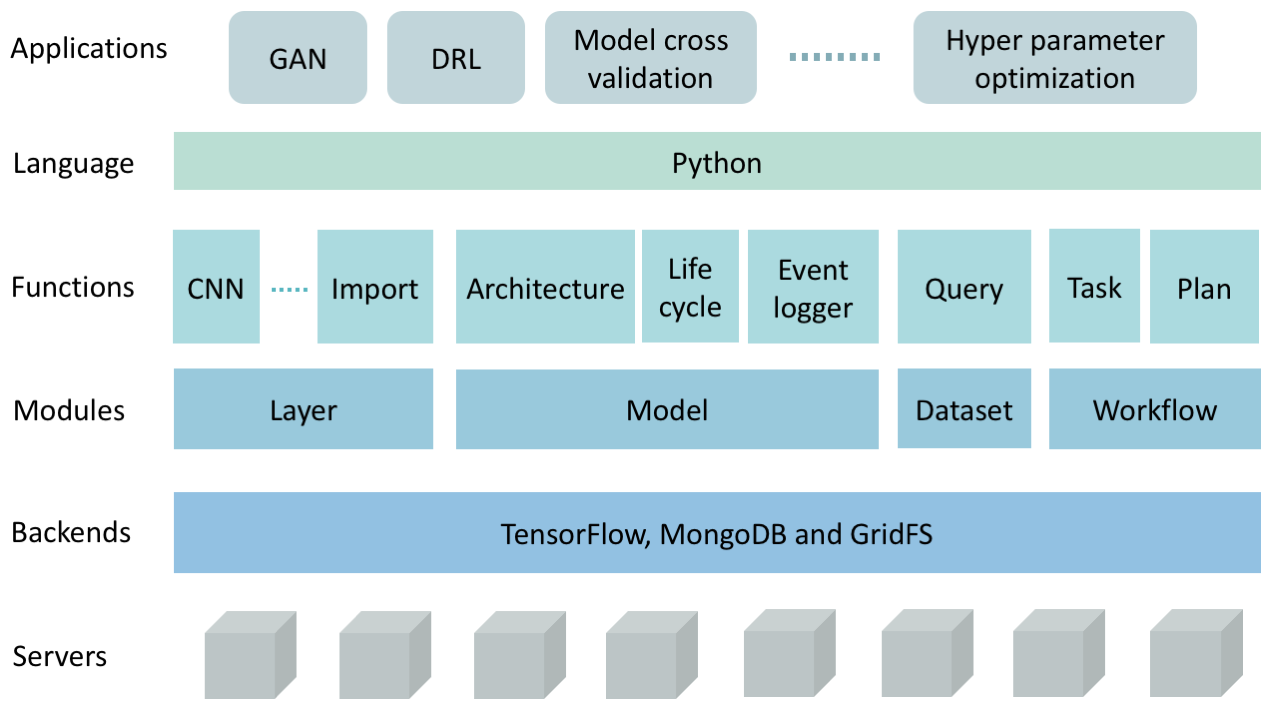
\includegraphics[scale=0.25, trim={0.3cm 0.5cm 0.3cm 0.3cm},clip]{figures/architecture}
	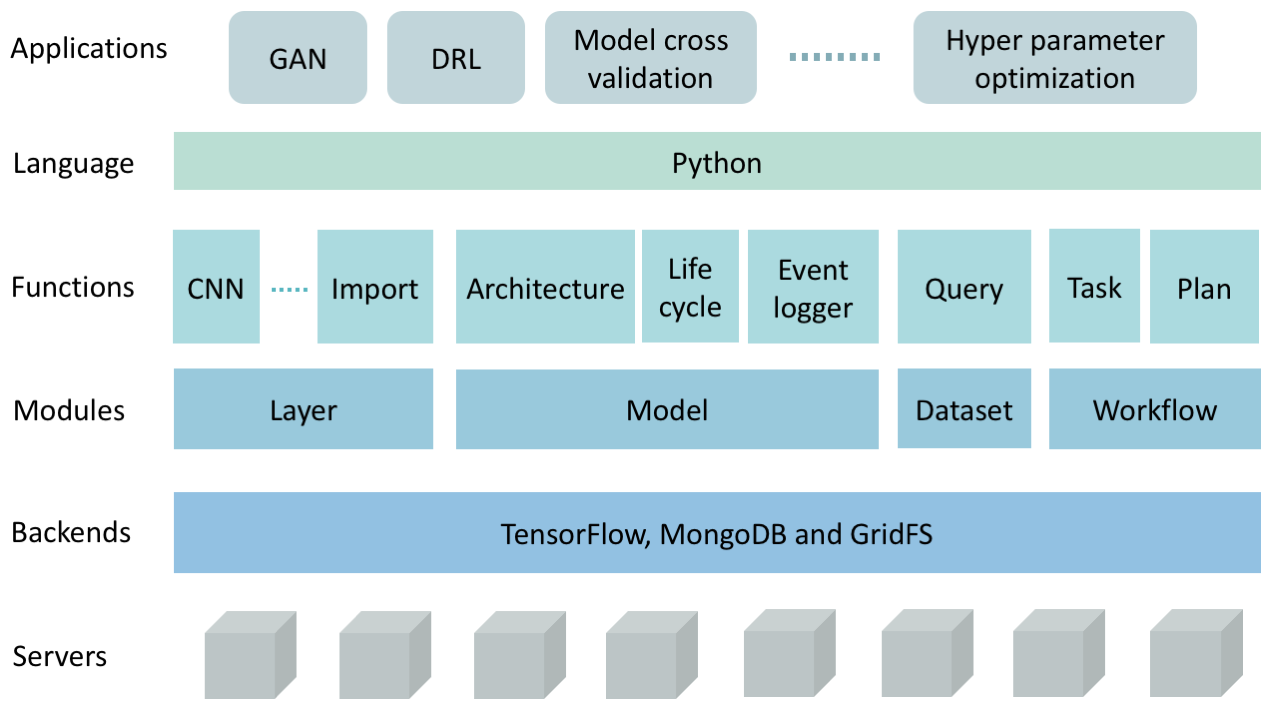
\includegraphics[scale=0.19, trim={0.3cm 0.5cm 0.3cm 0.3cm},clip]{figures/architecture.png}
	\caption{TensorLayer architecture.}
	\label{fig:architecture}
\end{figure} 

\subsection{Layer Module}

Layers are the core bricks of a neural network.
\tl provides a layer module that includes reference implementations of numerous layers, 
such as CNN, RNN, dropout, dropconnect, batch normalization and many others.
Layers are stacked to create a neural network with a declarative fashion, similar to
the extensively used Lasagne~\cite{lasagne}.
Each layer is given an unique key for  
helping developers achieve parameter sharing.
The networks are delegated to TensorFlow.
\tl inherits from TensorFlow to run on hybrid and distributed platforms. 
A concern towards \tl is performance overhead. We investigate this by
running classic models \cite{benchmark} using \tl and native TensorFlow implementations
on a Titan X Pascal GPU. Table~\ref{table:benchmark} shows that \tl exhibits negligible overhead in all models.

\begin{table}[]
	\centering
	\caption{TensorLayer (TL) and TensorFlow (TF) benchmark.}
	\label{table:benchmark}
	\begin{tabular}{|l|l|l|l|}
		\hline
		& CIFAR-10 & PTB LSTM & Word2vec \\ \hline
		TL & 2528 images/s     & 18063 words/s        & 58167 words/s    \\ \hline
		TF  & 2530 images/s    & 18075 words/s      & 58181 words/s   \\ \hline
	\end{tabular}
\end{table}


Layers can be flexibly composed and customized. 
They can be embedded with control functions 
that are lazily evaluated within TensorFlow to adjust training behaviours. This transparency design 
is favoured by \tl users, in particular when they are addressing domain-specific problems that 
require carefully customized models. 
In addition, to ease migration, \tl allows importing external layer and network implementations from other TensorFlow wrappers such as Keras, TFLearn and TFSlim by using the LambdaLayer.

\subsection{Model Module}

Model is the logical representation of a self-contained functional unit, and can be trained, evaluated and deployed in production. Each model has an unique network structure. During training, the model can have different versions or states (i.e., weights).
States can be persisted, cached and reloaded. We use MongoDB as the storage backend. 
Compared to other storage providers such as HBase or MySQL, MongoDB is out-of-box deployable,
simple to use, and rich in third-party management tools. In terms of performance,
it is able to achieve sufficient throughput for processing tensors 
which are the dominant data type in deep learning.

\tl supports recording user-defined model events. Conventional events reflect training steps, learning speed, and accuracy.
They are often used for diagnosing a training process in order to achieve, for example, model versioning~\cite{miao2017modelhub} and interactive learning~\cite{jiang2017interactive}. 

\subsection{Dataset Module}

The dataset module is used for managing training samples and prediction results. 
They are stored as documents in MongoDB. Each document contains a unique key, sample, label and user-defined tags.
Datasets are specified by declarative queries that carry conditions towards tag fields. 
Queries create views of underlying data, and thus do not cost extra storage.

Data are modelled as general streaming datasets. Each dataset is given a \emph{stream}
controller that constantly monitor the availability
of samples and predictions, and then trigger corresponding
training tasks towards this dataset. Intermediate training states are cached in memory
and later reloaded among batches.
The streaming abstraction is able to unify the declaration of offline and online data.
To speed up training efficiency, changes to a dataset is batched until
become significant.

\tl optimizes dataset performance thoroughly. Firstly, 
\tl creates indexes for frequently visited tags to accelerate
row selection. Secondly, datasets can be cached locally and partitioned to distribute workloads.
Thirdly, chunky data are compressed and sent in 
batches to improve I/O efficiency. Thirdly, in addressing
big blobs such as videos, \tl
adopts GridFS as the blob store.
In such a case, the rows in MongoDB carry pointers to the locations of sample blobs in GridFS. 
This two-layer storage architecture is transparent to developers. 

\subsection{Workflow Module}

The workflow module provides task abstraction to enable fault-tolerant asynchronous training. 
A training task is uniquely identified by 3-tuple: an input dataset key, a model key, and an output dataset key.
It is inserted into a task queue subscribed by an agent. An agent can
perform CPU / GPU training task or any user-defined function written in Python. Task completion messages are published onto a notification
queue subscribed by an agent master. 
This pub-sub system is naturally asynchronous. Multiple tasks can form a training plan to be scheduled by the master. Queues are persisted in the storage backend to ensure that failed tasks are replayed.

The workflow module simplifies the implementation of model group operations and learning systems that involves asynchronous feedback loops in operation. It is also 
useful for complex cognitive systems
that have training dependency among components. 
For example, the developer of an image captioning system \cite{showandtell2015} first trained
a CNN to understand the context of images, and then trained a
RNN decoder to generate description based on recognized context. This example
thus forms a two-stage asynchronous training plan that can be supported by \tl.





















\section{Applications}
\label{sec:experiment}


\begin{figure}
	\centering% trim={<left> <lower> <right> <upper>}
%	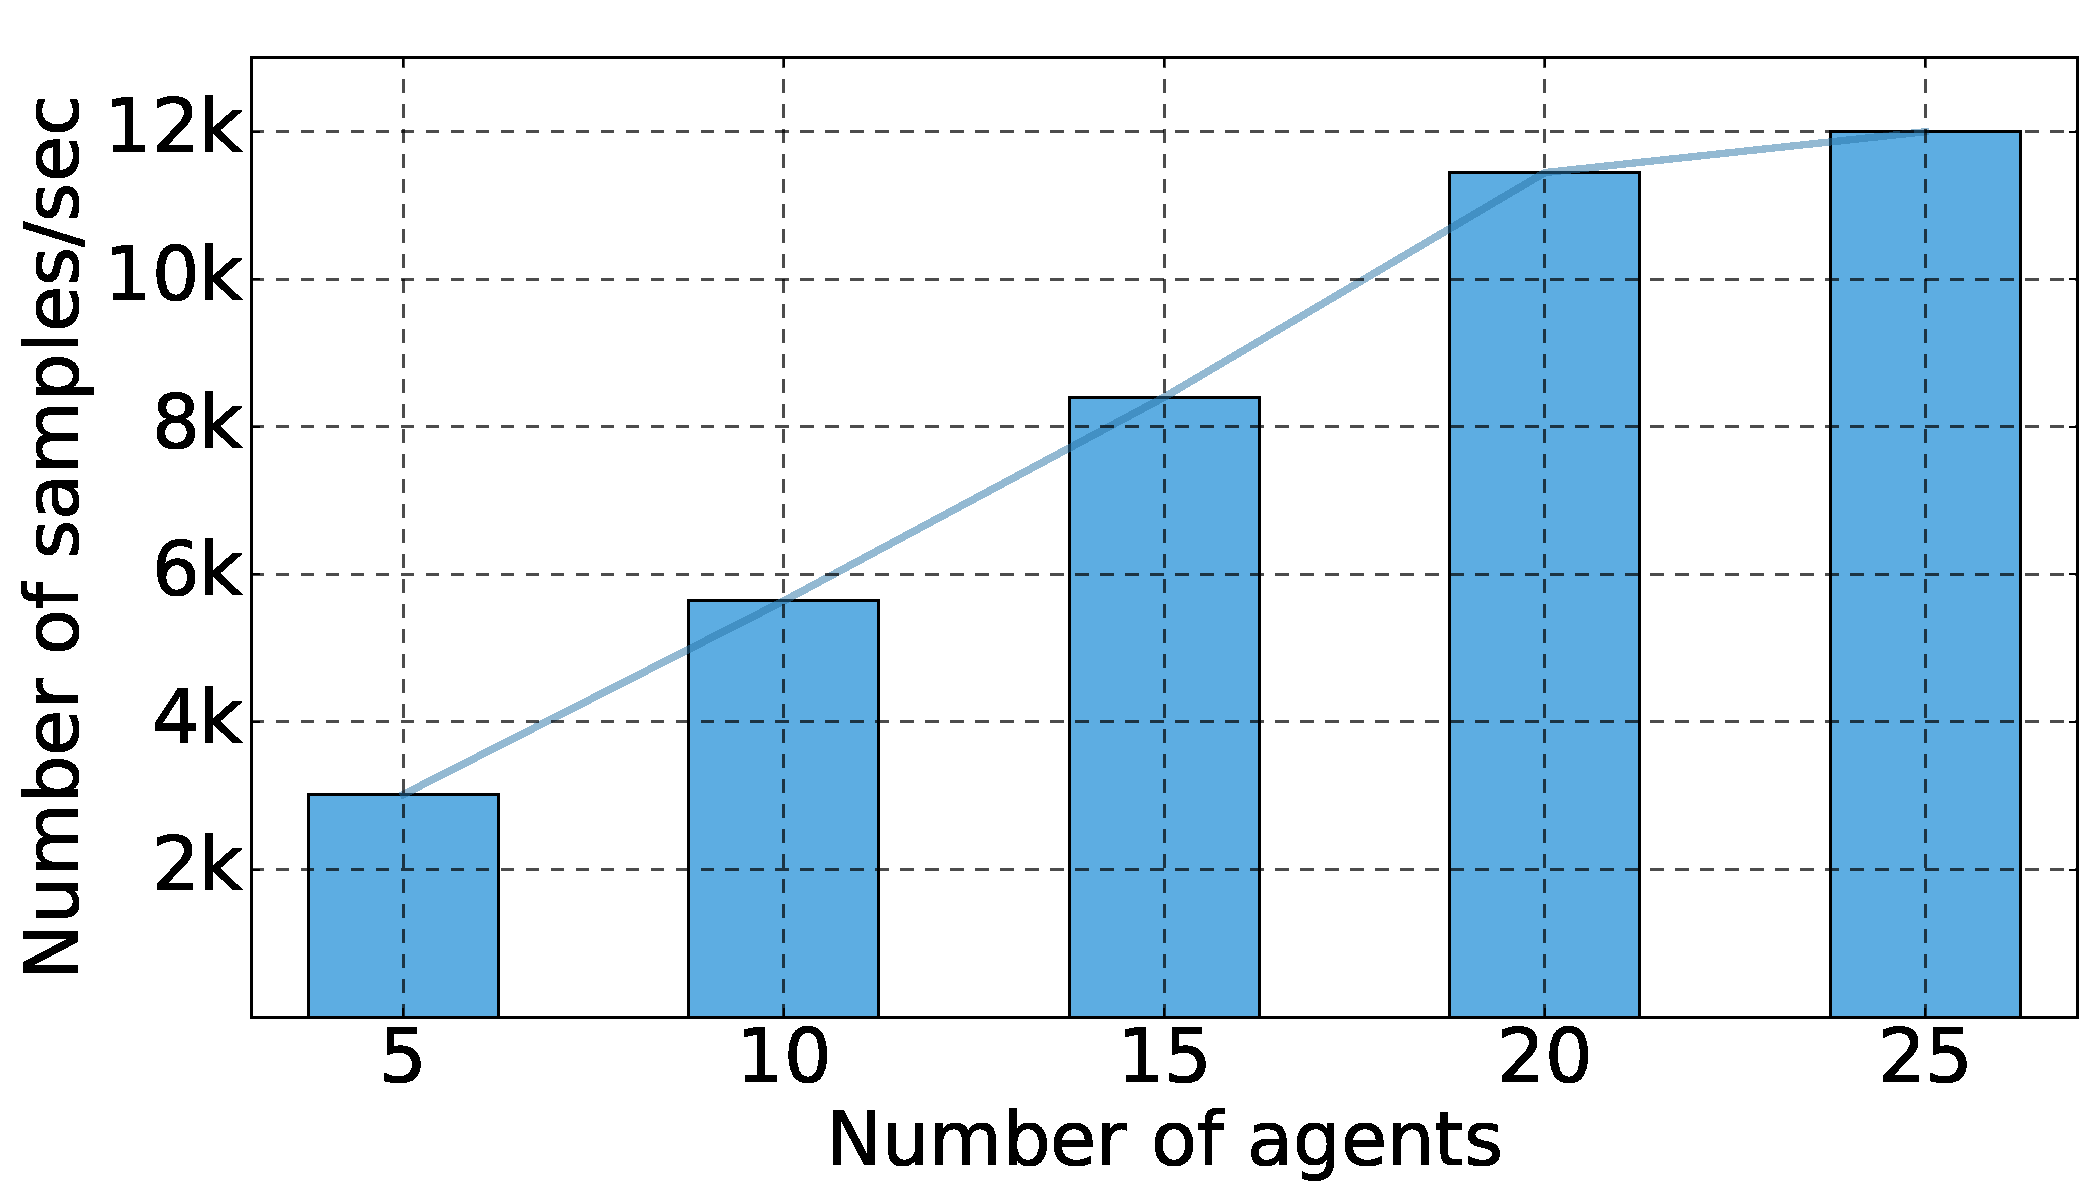
\includegraphics[width=0.42\textwidth]{figures/evaluation/drl_results2}
%		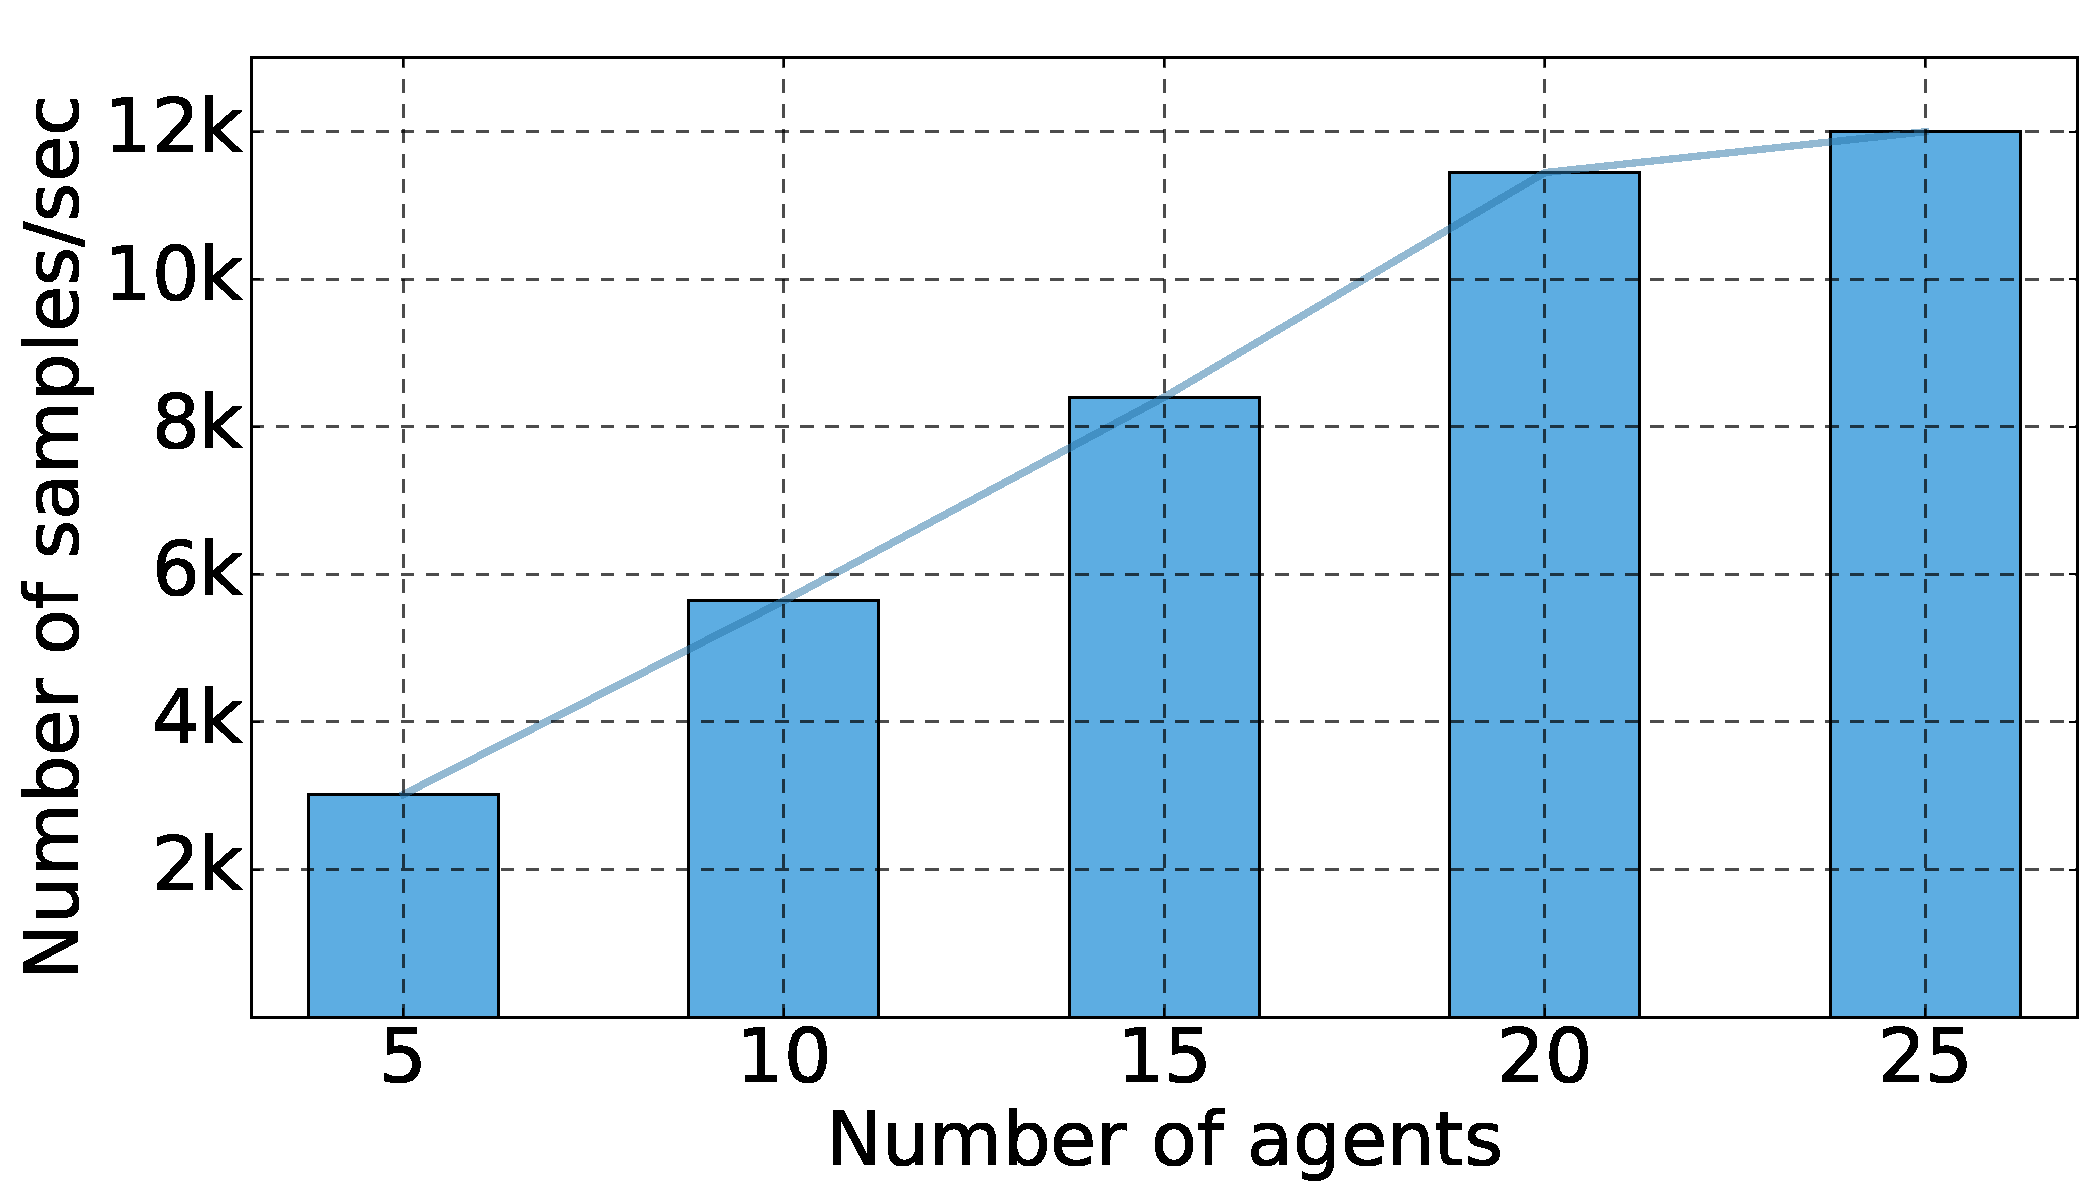
\includegraphics[scale=0.23, trim={0cm 0.39cm 0cm 1.cm},clip]{figures/evaluation/drl_results2}
		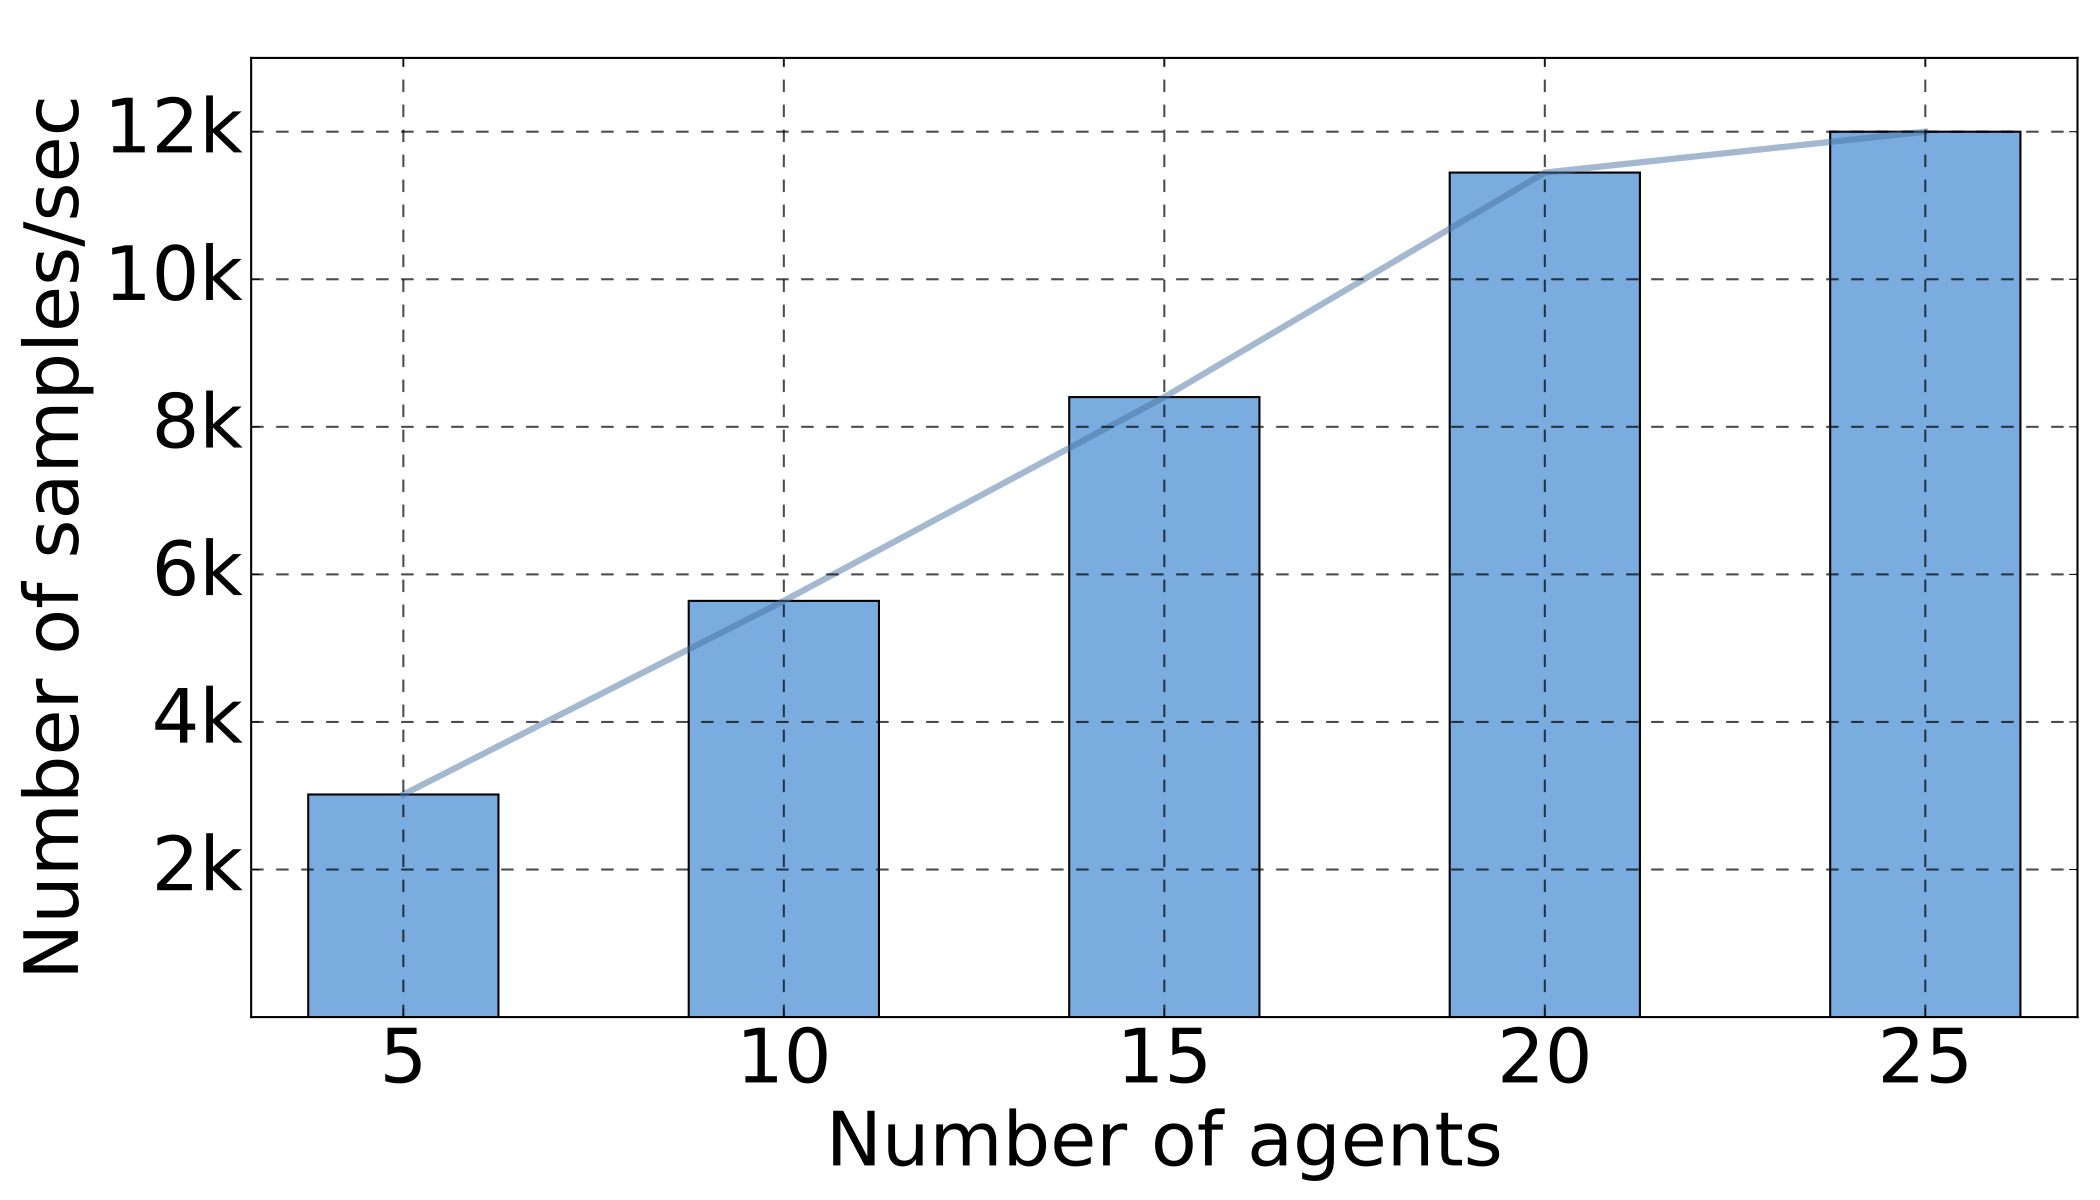
\includegraphics[scale=0.19, trim={0cm 0.39cm 0cm 1.cm},clip]{figures/evaluation/drl_results2.png}
	\caption{Training throughput vs. number of agents used for generating training samples.}
	\label{fig:drl_results}
\end{figure} 

\begin{figure}
	\centering   % trim={<left> <lower> <right> <upper>}
	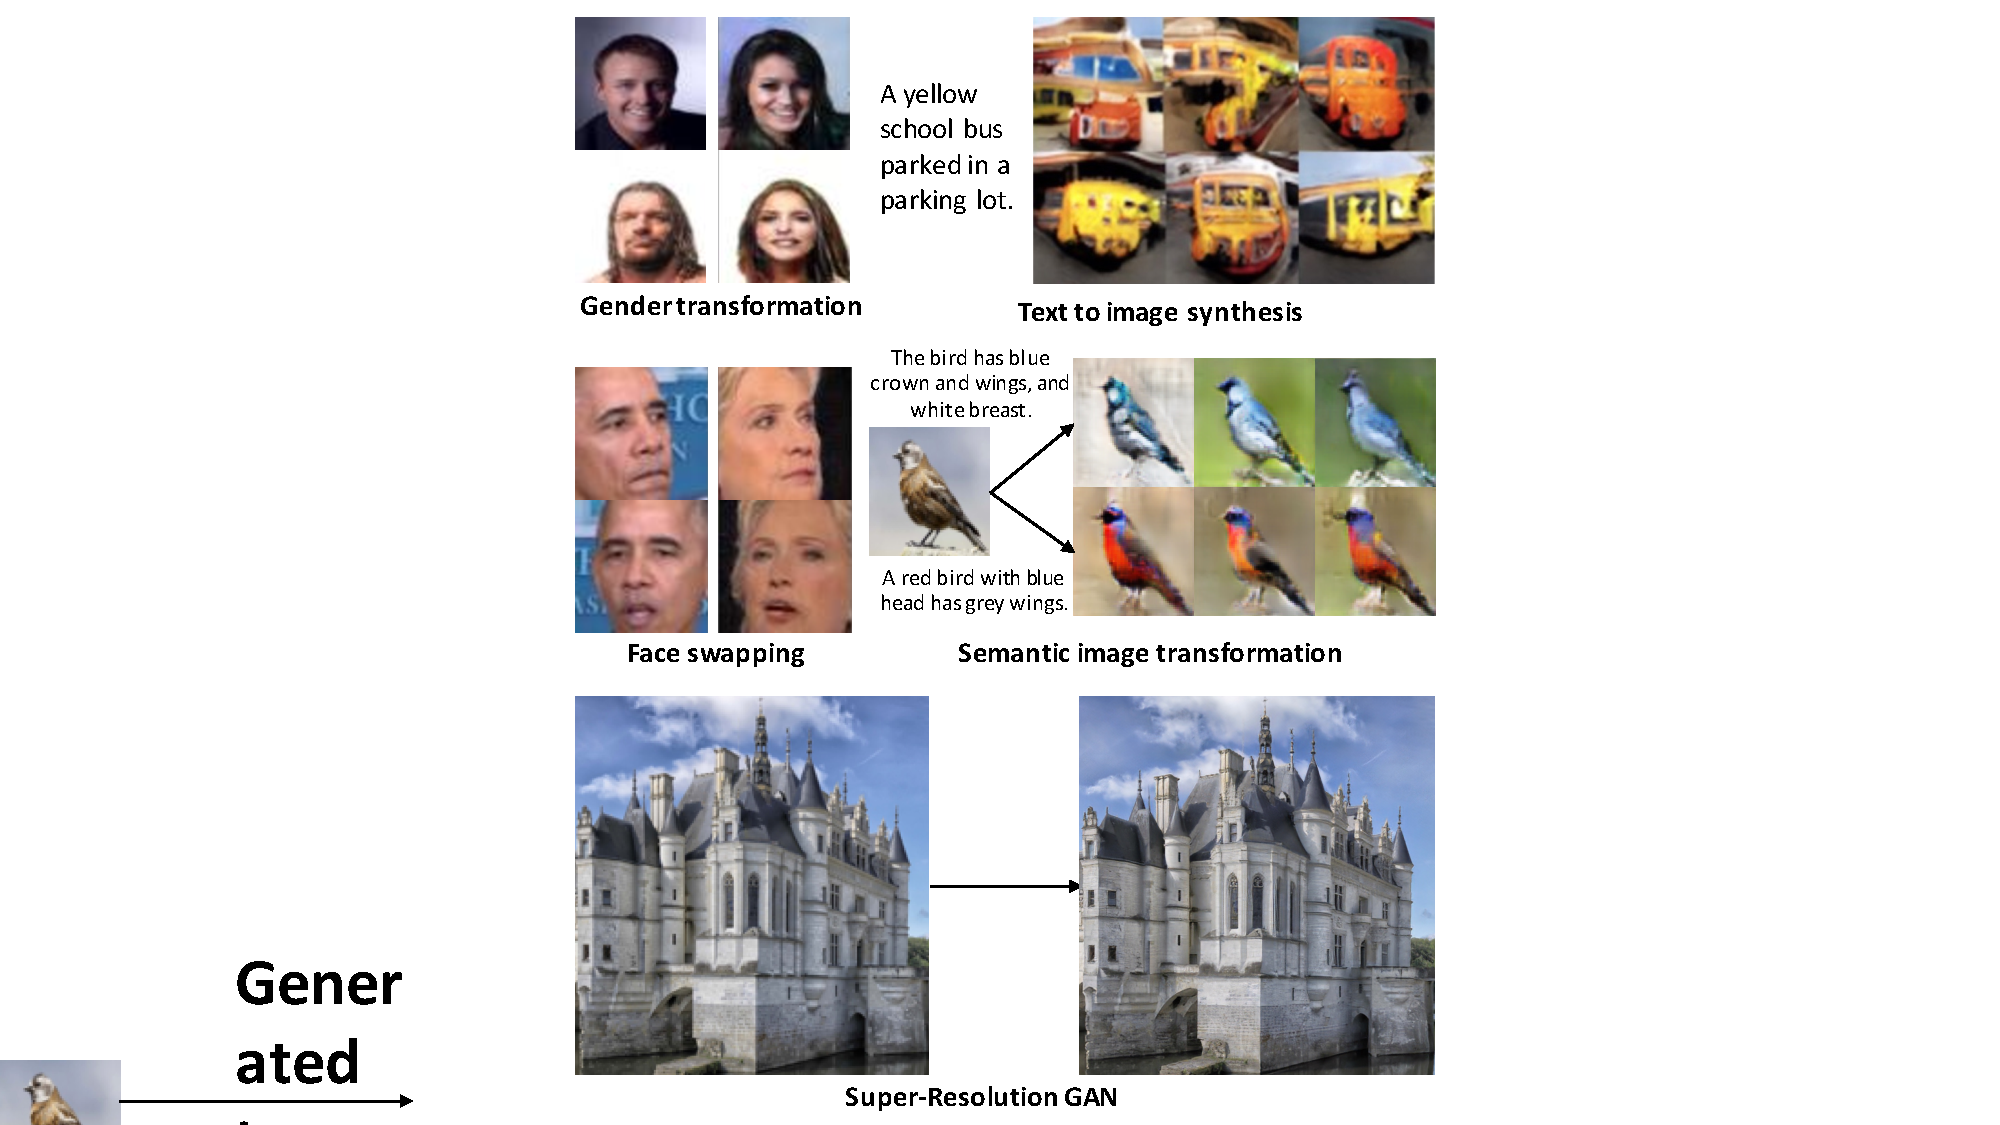
\includegraphics[scale=0.48, trim={9.5cm 0.2cm 9.5cm 0.2cm},clip]{figures/more_app4}
%	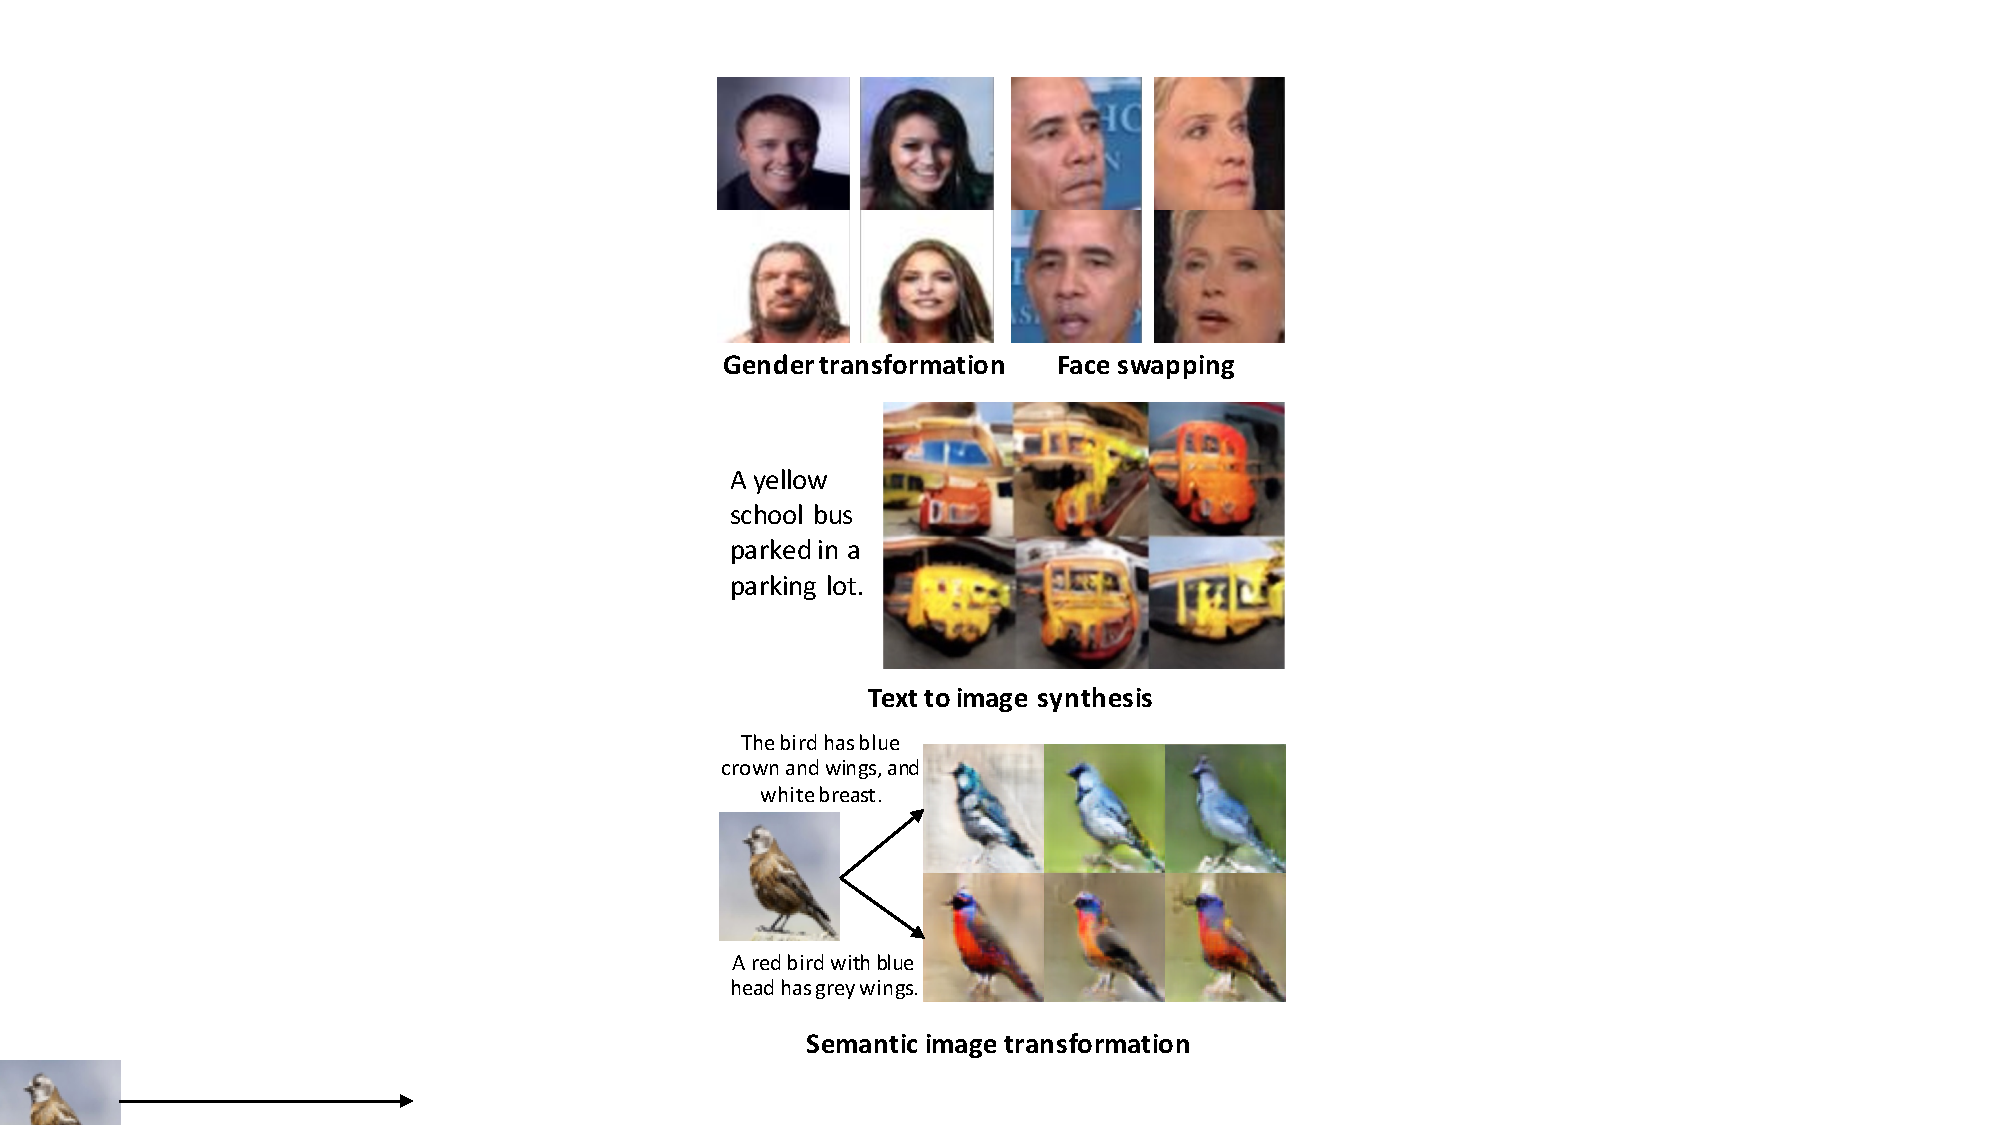
\includegraphics[scale=0.8, trim={12cm 1.0cm 12cm 1.0cm},clip]{figures/more_app3}
	%	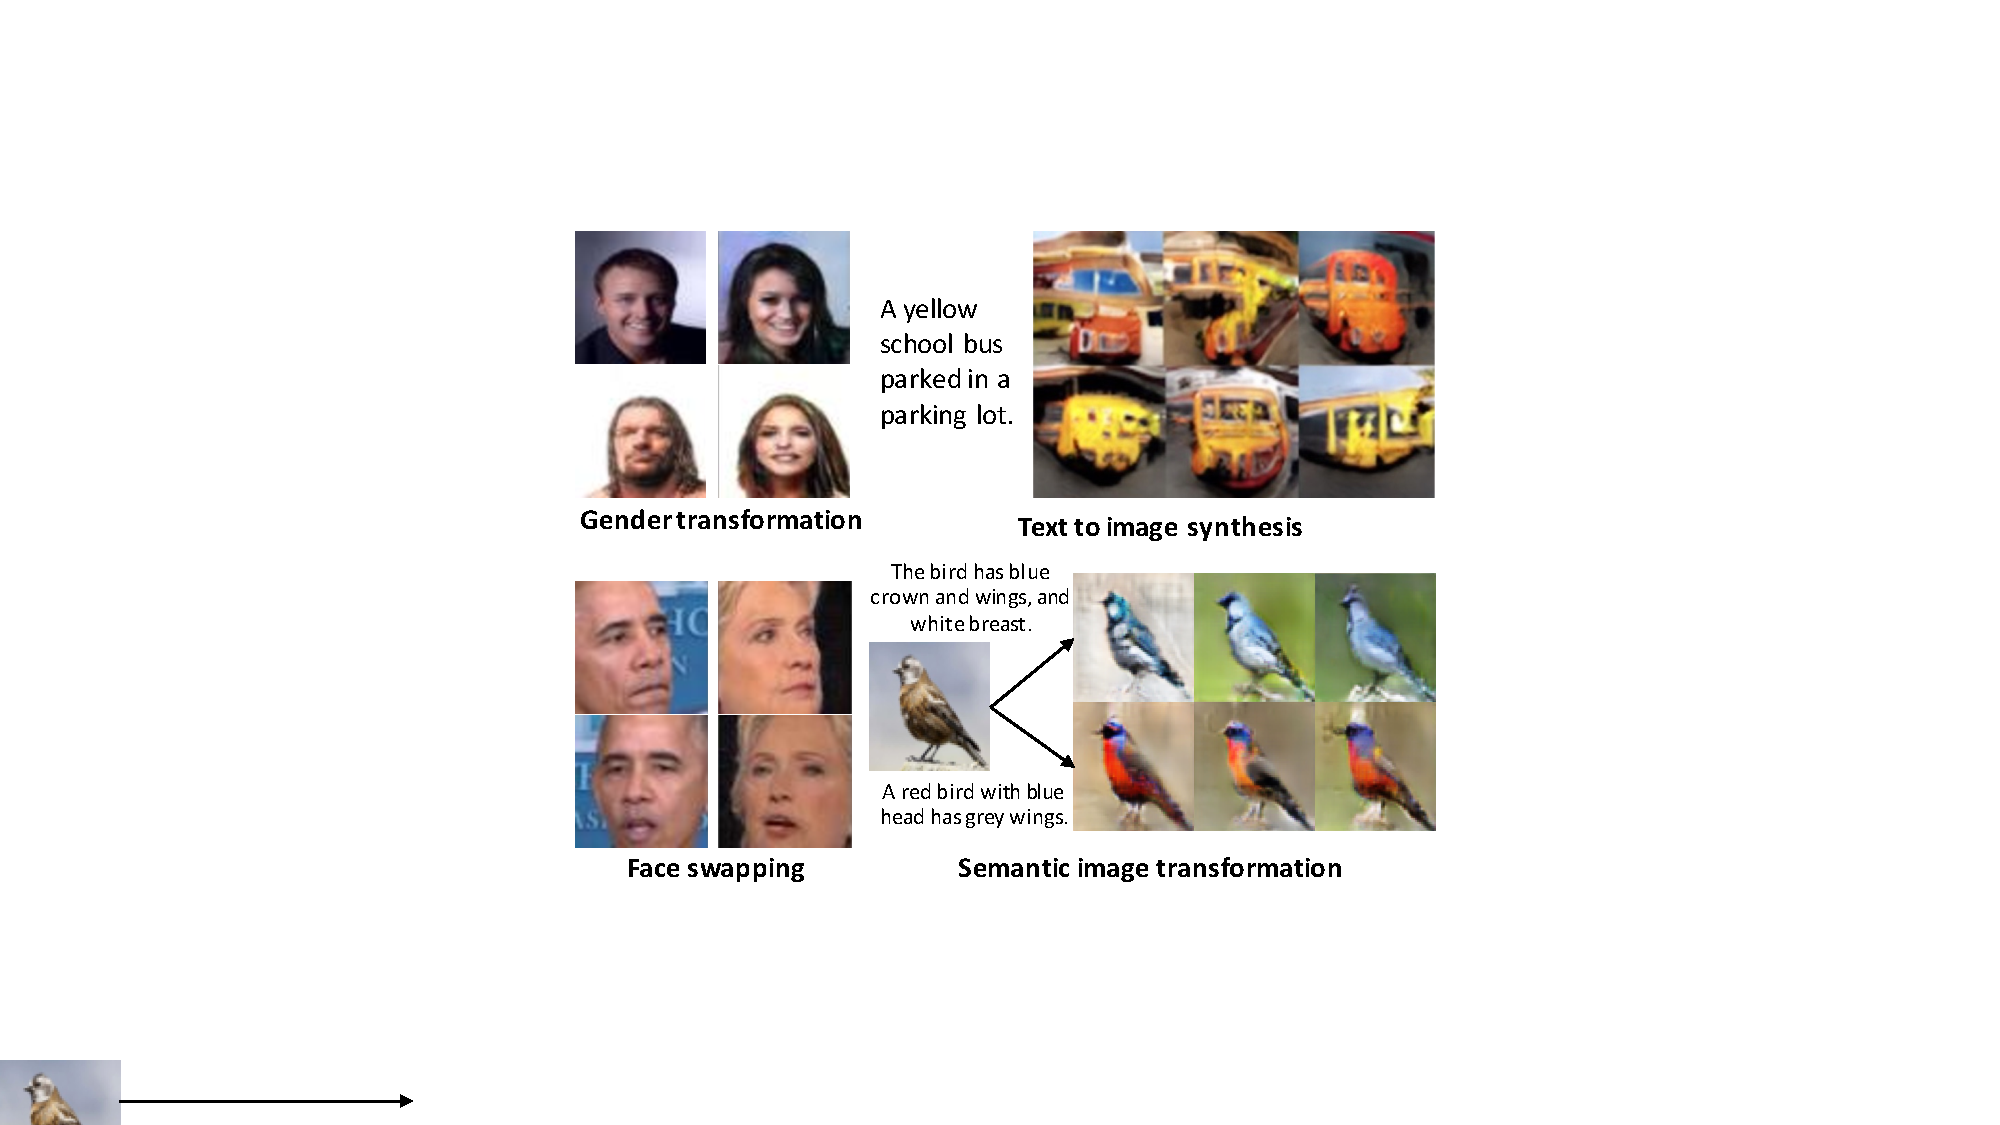
\includegraphics[scale=0.57, trim={9.5cm 4.0cm 9.5cm 4.0cm},clip]{figures/more_app3_2}
	\caption{Highlighted \tl applications.}
	\label{fig:more_app}
\end{figure} 
%\begin{figure*}[h!]
%	\centering   % trim={<left> <lower> <right> <upper>}
%	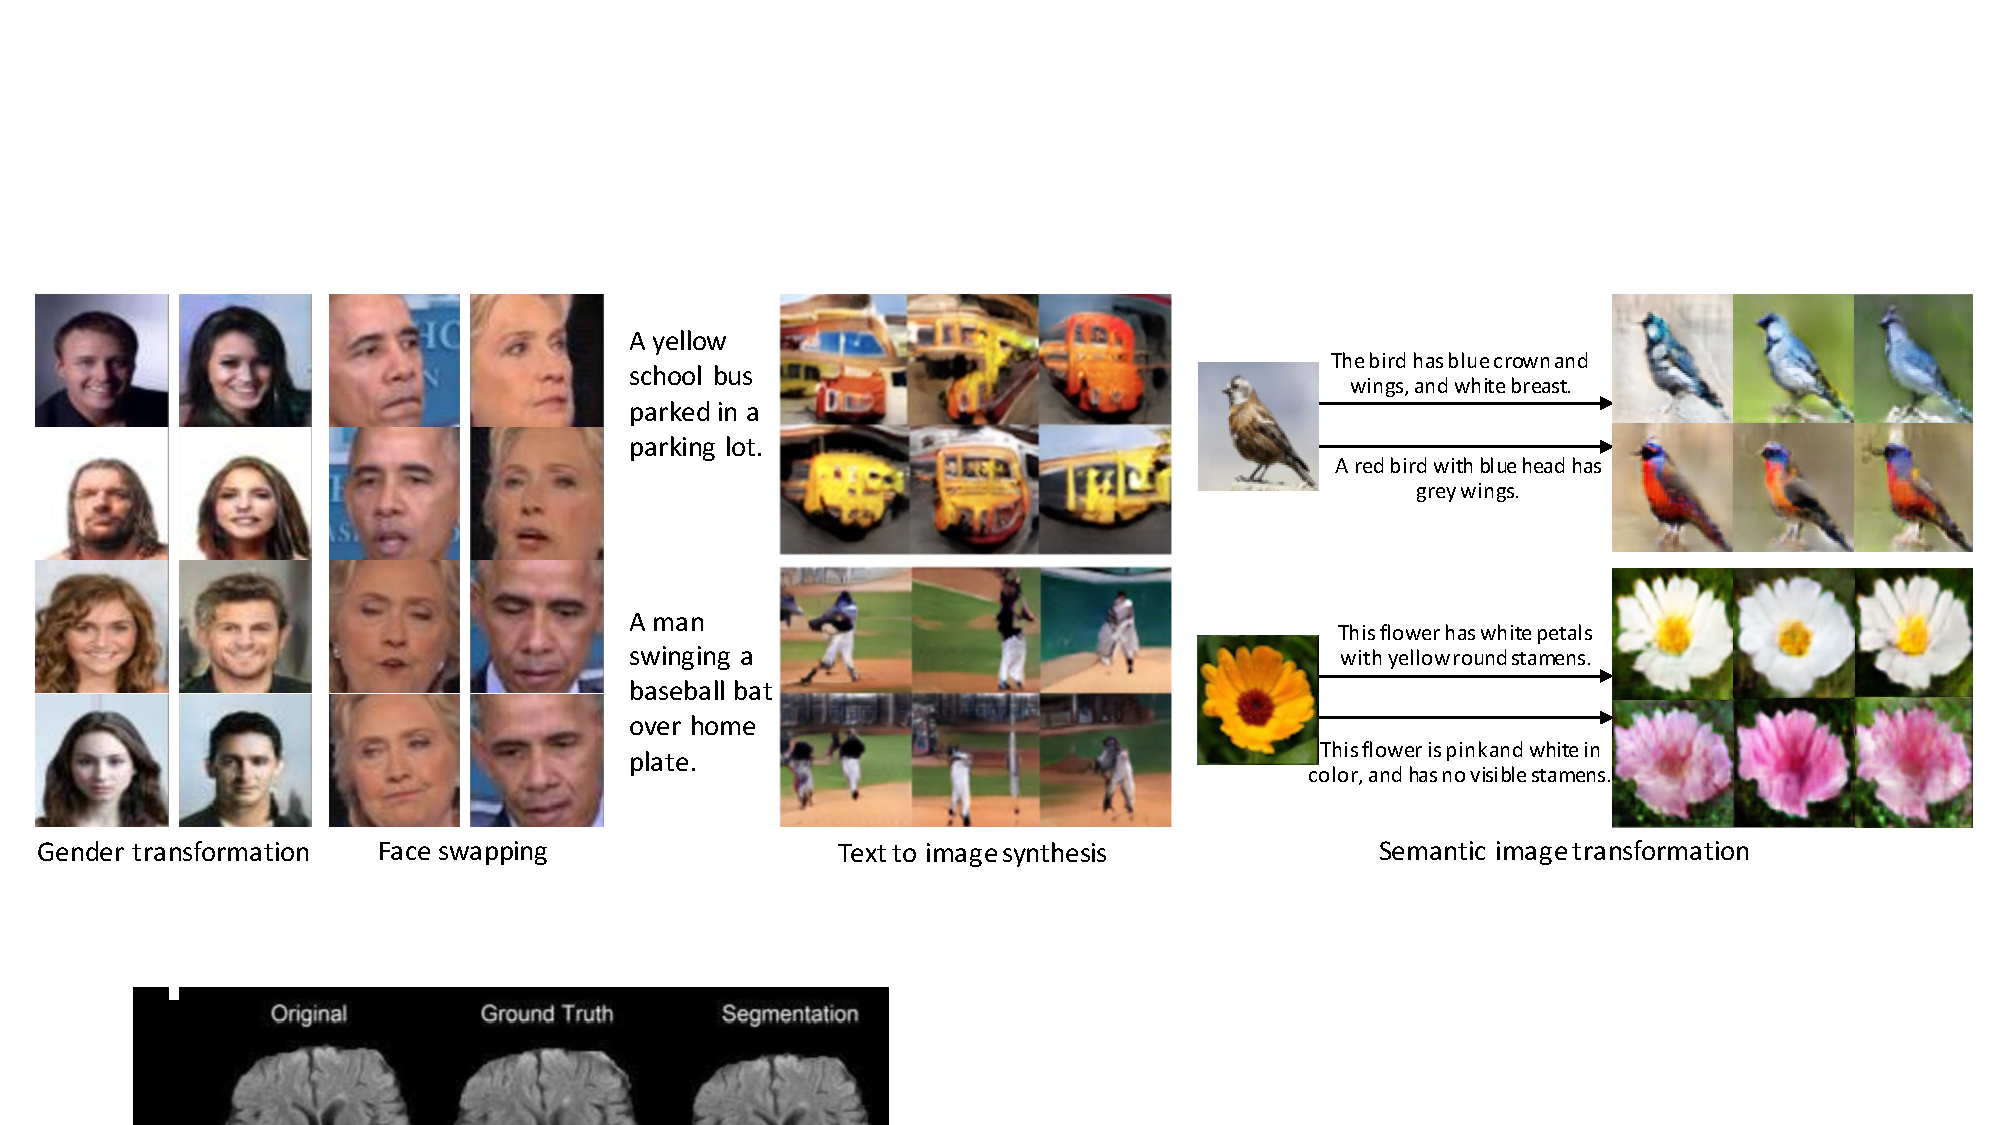
\includegraphics[scale=0.5, trim={0cm 4.0cm 0cm 3.0cm},clip]{figures/more_app}
%	\caption{Highlighted \tl applications.}
%	\label{fig:more_app}
%\end{figure*} 

This section presents a comprehensive study of
deep learning applications that can benefit from using \tl in terms of development efficiency. 
%In this section, we demonstrate some examples that show the advantages of TensorLayer, and some research projects using TensorLayer in Imperial College London. 
Relevant source code is %hosted by a public repository~\footnote{\url{https://github.com/akaraspt/tl\_paper}}.
publicly available on Github~\footnote{\url{https://github.com/akaraspt/tl\_paper}}.

\textbf{Generative adversarial networks.}
%GANs are increasingly popular in multimedia tasks.  %~\cite{radford2015dcgan} 
%A GAN is a dynamic neural network that has two input sources at the discriminator. 
GANs have become a popular deep learning based generative framework for multimedia tasks.
The discriminator network of GANs has two source inputs, which is different from common deep learning architectures. 
\tl enables developers to efficiently construct network architectures of GANs, 
and control the dynamics of a training process, and achieve parameter optimization. 
We take DCGAN~\cite{radford2015dcgan}, an image generation network, 
as an instance to evaluate the helpfulness of \tl. While achieving identical training efficiency, \tl implementation has 187 lines of code (LOC), 
which is 75\% smaller than the published TensorFlow implementation (746 LOC). 
% ours : main.py 96 model.py 67 utils.py 24  / download.py 136
% carpedm20: main.py 76  model.py 406  ops.py 83  utils.py 181 / download.py 147
We use Super-Resolution GAN (SRGAN)~\cite{Ledig2016srgan} as another example. The TensorLayer-based implementation of SRGAN is 526 LOC in length. This is smaller than many other open-sourced implementations that often have more than a thousand LOC.


\textbf{Deep reinforcement learning.} A DRL application is a great example that showcases a joint usage of the layer, model, dataset and workflow modules. 
Specifically, developers can use \tl to build a DRL model, manage model's states between iterations, and create training data that will be constantly generated by concurrent game players.
To demonstrate this, we implement a distributed asynchronous DRL system %~\cite{mnih2016asynchronous}\
 in a cluster that has 10 Gbps connectivity. 
The system trains an agent for playing Atari pong game~\cite{pingpixel2016} on a GTX 980 GPU.
The trainer keeps receiving samples (i.e., observations, actions and rewards)
from game players simulated by \tl agents. 
Trained network models are shared with all players %using the model synchronization function in \tl. 
via the model module of \tl.
Figure~\ref{fig:drl_results} illustrates the scalability of \tl in powering such a system. The training throughput is linearly increasing with more joining agents, until %the GPU finally becomes the bottleneck.
it reaches the maximum capacity of the GPU. 



\textbf{Hyper parameter optimization and cross-validation.}
These two machine learning jobs are necessary for addressing domain-specific problems, 
e.g., medical signal processing~\cite{deepsleepnet2017}, which usually
do not have universally effective models. Hence, they
help developers explore various models and evaluate their performance.
Previously, they were implemented using ad-hoc components. These implementations incurred high maintenance cost, 
and reduced task efficiency due to the cross-component overhead (e.g., serialization and network transfer).
Integrating them with \tl significantly reduces the development and maintenance complexity. 
In addition, experiment results show that \tl can gently increase task parallelism while only incurring
low memory and I/O overhead within the shared data infrastructure. 



\textbf{More applications.}
There are many more applications that have benefited from using \tl. We highlight a few of them here:
multi-model research~\cite{i2t2i2017}, image transformation~\cite{unsupim2im2017, myiccv2017}, and medical signal processing~\cite{braintumor2017, deepsleepnet2017}.
Their results are illustrated in Figure~\ref{fig:more_app}.







\section{Availability}
TensorLayer is open sourced under the license of Apache 2.0.
It can be used in Linux, Mac OS and Windows environments.
\tl has a low adoption barrier. It provides a multilingual documentation, massive tutorials and thorough examples, such as CNNs (like VGG, ResNet, Inception), text-related applications (like text generation, Word2vec, machine translation, image captioning), GANs (text-to-image synthesis, CycleGAN, stackGAN, SRGAN), reinforcement learning algorithms (like Deep Q-Network, Policy Gradients, Asynchronous Advantage Actor-Critic (A3C)) and etc.

\section{Acknowledge}
We would like to thank TensorLayer Open Source Community for numerous fruitful discussions. We also appreciate the feedbacks from Biye Jiang affiliated with University of California Berkeley.
%{\color{blue}Hao Dong, Akara Supratak, Luo Mai, Axel Oehmichen and Simiao Yu are supported by the OPTIMISE Portal, the Faculty of Information and Communication Technology of Mahidol University (MUICT), the Google Fellowship in Cloud Computing, the Innovation Medicines Initiative (IMI) eTRIKS project and Jaywing plc respectively.}
Hao Dong is supported by the OPTIMISE Portal. Akara Supratak is supported by the Faculty of Information and Communication Technology, Mahidol University (MUICT). Luo Mai is supported by a Google Fellowship in Cloud Computing. Axel Oehmichen is supported by the Innovation Medicines Initiative (IMI) eTRIKS project. Simiao Yu is supported by Jaywing plc. 




\bibliographystyle{ACM-Reference-Format}
\bibliography{reference} 

\end{document}
